\documentclass[a4paper,10pt]{report}
\usepackage{Cours}
\usepackage{delarray}
\usepackage{fancybox}
\newcommand{\Sum}[2]{\ensuremath{\textstyle{\sum\limits_{#1}^{#2}}}}
\newcommand{\Int}[2]{\ensuremath{\mathchoice%
	{{\displaystyle\int_{#1}^{#2}}}
	{{\displaystyle\int_{#1}^{#2}}}
	{\int_{#1}^{#2}}
	{\int_{#1}^{#2}}
	}}
\usepackage{pstricks-add}



\begin{document}
% \everymath{\displaystyle}

\maketitle{Chapitre 16}{Variables aléatoires discrètes}
\noindent Dans tout ce chapitre, $(\Omega, \A, \P)$ désigne un espace probabilisé quelconque. On généralise dans ce chapitre ce qui a été étudié dans le chapitre lié aux variables aléatoires finies en première année.


\section{Généralités}
\subsection{Introduction}

\noindent Considérons l'expérience suivante : on jette deux fois un dé et on s'intéresse à la somme des chiffres obtenus que l'on note $S$. Modélisons cette expérience de la manière suivante : chaque issue de l'expérience peut être représentée par un couple $(x,y)$ où $x \in$ $\Interv16$ et $y  \in$ $\Interv16$. Autrement dit l'univers peut s'écrire $\Omega = \Interv16^2$ et nous sommes en situation d'équiprobabilité.
%
%\vspace{0.2cm}
%
%\noindent Étant donné que l'on s'intéresse à la somme des chiffres obtenus, de quelle manière commode peut-on représenter la situation ? 

\vspace{0.2cm}

\noindent La somme $S$ est en fait une \og \textit{variable} \fg  qui varie \textit{aléatoirement} selon le couple obtenu. On dit que c'est une variable aléatoire. Remarquons que $S$ associe à chaque issue de l'expérience $\omega=(x,y)$ un chiffre (la somme des chiffres obtenus) : c'est une application de $\Omega$ dans $\mathbb{R}$.

\vspace{0.2cm}

\noindent Pour finir, remarquons que ce qui nous intéresse, c'est la somme des chiffres obtenus et non pas les chiffres obtenus. On s'intéressera par exemple par la suite à la probabilité que cette somme soit égale, inférieure, supérieure à un certain réel.

\subsection{Définition}
\begin{defin}
Une \textit{variable aléatoire discrète} sur $(\Omega, \mathcal{A})$ est une application définie sur $\Omega$ dont l'image est finie ou dénombrable et telle que l'image réciproque par $X$ de tout élément de $X(\Omega)$ appartient à $\mathcal{A}$.
\end{defin}
Autrement dit,
\begin{itemize}
\item $X(\Omega)$, qui est l'ensemble des valeurs que prend la variable aléatoire $X$, défini par :
$$  X(\Omega) = \{X(\omega), \, \omega \in \Omega\} $$
est fini ou dénombrable.
\item Pour tout $x \in X(\Omega)$, $X^{-1}(\lbrace x \rbrace) \in \mathcal{A}$ (c'est un évènement).
\end{itemize}

\medskip

\begin{notas}
\item On dit que $X(\Omega)$ est le \textit{support} (ou l'\textit{ensemble-image}) de $X$.
\item Si $x \in X(\Omega)$, on note $[X = x]$ ou $(X=x)$ l'ensemble $\lbrace \omega \in \Omega, \, X(\omega)=x \rbrace$.
\item Si $X$ est à valeurs réelles, on note $[X \leq x]$ ou $(X \leq x)$ l'ensemble $\lbrace \omega \in \Omega, \, X(\omega) \leq x \rbrace$. On définit de même $[X>x]$ et $[X<x]$ ou encore $[X \geq x]$.
\item Plus généralement, si $U \subset X(\Omega)$, on note :
$$[X\in U] = X^{-1}(U)= \lbrace \omega \in \Omega, \, X(\omega) \in U \rbrace$$
\end{notas}

\begin{ex} Reprenons l'exemple de l'introduction. Le support de $S$ est $S(\Omega) = \Interv{2}{12}$. L'évènement $[S=11]$ est réalisé si et seulement si la somme des deux numéros obtenus vaut $11$. On a :
\[ [S=11] = \lbrace (5,6), (6,5) \rbrace\]
\end{ex}

\begin{ex} On lance un dé jusqu'à obtenir un 6. $T$ vaut $k$ si le jeu se termine en $k$ lancers exactement, $T$ vaut 0 si le jeu ne se termine jamais. Déterminons le support de $T$. Cette variable est-elle discrète ?

\vspace{2cm}
\end{ex}

\begin{prop} Soit $X$ une variable aléatoire sur $(\Omega, \mathcal{A})$ et $U$ un sous-ensemble de $X(\Omega)$. Alors $X^{-1}(U) \in \mathcal{A}$.
\end{prop}


\begin{rems}
\item Si $X$ est une variable aléatoire discrète alors $X(\Omega)$ est fini ou dénombrable donc on peut écrire $X(\Omega)$ sous la forme :
$$ X(\Omega) = \lbrace x_n \, \vert \, x_n \in I \rbrace$$
où $I$ est une partie (finie ou infinie) de $\mathbb{N}$. Dans tout le chapitre, on considérera que les $x_n$ sont \textbf{distincts}.
\item Si $\Omega$ est fini, $X(\Omega$) aussi et les conditions pour être une variable aléatoire sont vérifiées car $\mathcal{A}= \mathcal{P}(\Omega)$. Dans ce cas, toute application de $\Omega$ dans $\mathbb{R}$  est une variable aléatoire sur $(\Omega, \mathcal{P}(\Omega), \P)$.
\end{rems}

%\begin{ex}
%On lance un dé jusqu'à obtenir un 6. $T$ vaut $k$ si le jeu se termine en $k$ lancers exactement, $T$ vaut 0 si le jeu ne se termine jamais. Déterminons le support de $T$. 
%\end{ex} 

%\begin{defip} 
%Soit $X$ est une variable aléatoire réelle discrète. Alors $\dis \big([X=x]\big)_{x\in X(\Omega)}$  est un système complet d'événements appelé \textit{système complet d'événements associé à la variable aléatoire discrète $X$}. En particulier :
%\[ \sum_{x\in X(\Omega)} \P(X=k) = 1 \]
%\end{defip}
%
%\begin{att} La somme peut être finie ou la somme d'une série convergente.
%\end{att}
%
%\begin{rem}
%Le système complet d'évènements associé à une variable aléatoire $X$ permet de calculer la probabilité d'un événement à l'aide de la \textit{formule des probabilités totales}, en distinguant plusieurs cas selon les valeurs possibles de $X$.
%\end{rem}

\section{Loi de probabilité d'une variable aléatoire réelle discrète}
\subsection{Définition et exemples}

\begin{defin}[Loi d'une variable aléatoire]
Soit $X$ une variable aléatoire sur $(\Omega, \mathcal{A}, \P)$. On appelle \textit{loi de la variable aléatoire} $X$ la fonction définie sur $X(\Omega)$ par :
$$ \forall x \in X(\Omega), \, P_X(x) = P(X=x)$$
\end{defin}
\noindent Ainsi, déterminer la \textit{loi de probabilité} d'une variable aléatoire discrète $X$ c'est : 
 \begin{itemize}
  \item Déterminer le support $X(\Omega)$ : c'est-à-dire toutes les valeurs possibles de $X$.
  \item Calculer les probabilités $\P\big(X=k\big)$ pour toutes les valeurs de $k$ appartenant à $X(\Omega)$.
 \end{itemize}

\medskip

\begin{rem} La loi de $X$ définit ainsi une probabilité sur $(X(\Omega), \mathcal{P}(X(\Omega)))$ : l'univers n'est \og plus important \fg, on s'intéresse aux valeurs de $X$.
\end{rem}

\begin{ex} Une urne contient 1 boule rouge, 2 noires et 2 jaunes. On tire successivement et sans remise une boule jusqu'à ce qu'il ne reste que deux couleurs. Soit $X$ le nombre de tirages nécessaires. Déterminons la loi de $X$.

\vspace{10cm}
\end{ex}

\begin{ex} On lance un dé équilibré jusqu'à obtenir un 6. $T$ vaut $k$ si le jeu se termine en $k$ lancers exactement, $T$ vaut 0 si le jeu ne se termine jamais. Déterminons la loi de $T$.

\vspace{10cm}
\end{ex} 

\newpage

$\phantom{test}$

\vspace{6cm}

\begin{exa} Soit $n \in \mathbb{N}$. Une urne contient 2 boules blanches et $n$ boules rouges. On tire au hasard une boule dans l'urne et on recommence (sans remise) jusqu'à temps d'obtenir une boule blanche. On appelle $X$ le rang de sortie de la première boule blanche et $Y$ le nombre de boules rouges restantes à ce moment dans l'urne. Déterminer la loi de $X$ et exprimer $Y$ en fonction de $X$.
\end{exa} 


\begin{prop} Soit $X$ une variable aléatoire discrète sur $(\Omega, \mathcal{A}, \P)$. On écrit alors :
$$ X(\Omega)= \lbrace x_n \, \vert \, n \in I \rbrace$$
où $I$ est une partie de $\mathbb{N}$. Pour tout $U \subset X(\Omega)$, on a :
$$ \P(X \in U) = \sum_{x_n \in U} \P(X=x_n)$$
\end{prop}

\begin{rem} La somme peut être une somme finie ou alors la somme d'une série convergente. Dans le cas d'une somme de série convergente, on admet que l'ordre de la sommation n'est pas important.
\end{rem}

\begin{preuve} 

\vspace{3cm}
\end{preuve}

\begin{ex} Si $X(\Omega) = \mathbb{N}$, la probabilité que $X$ soit paire est :
$$ P(\hbox{\og X est paire \fg }) = \sum_{n=0}^{+ \infty} P(X=2n)$$
\end{ex}

\begin{cor} Soit $X$ est une variable aléatoire discrète sur $(\Omega, \mathcal{A}, \P)$.  On écrit alors :
$$ X(\Omega)= \lbrace x_n \, \vert \, n \in I \rbrace$$
où $I$ est une partie de $\mathbb{N}$. Alors $\dis \big([X=x_n]\big)_{n \in I}$  est un système complet d'événements appelé \textit{système complet d'événements associé à la variable aléatoire discrète $X$}. En particulier :
$$\sum_{n \in I} \P(X=x_n) = 1$$
\end{cor}

\medskip

\noindent Ce dernier résultat est très utilisé avec la formule des probabilités totales : pour tout évènement $B$,
$$ \P(B) = \sum_{n \in I} P(X=x_n) P_{(X=x_n)}(B)$$

\subsection{Fonction de répartition}


\begin{defin}[Fonction de répartition]
Soit $X$ une variable aléatoire \textit{réelle} discrète sur $(\Omega, \mathcal{A}, \P)$. On appelle \textit{fonction de répartition} de $X$ la fonction notée $F_X$ définie pour tout $x \in \mathbb{R}$ par :
$$F_X(x) = \P(X \leq x) $$
\end{defin}


\begin{prop}
Soient $X$ une variable aléatoire réelle discrète sur $(\Omega, \mathcal{A}, \P)$ et $F_X$ sa fonction de répartition.
\begin{itemize}
\item Pour tout $ x \in \mathbb{R}$, $F_X(x) \in [0,1]$
\item $F_X$ est une fonction croissante sur $\mathbb{R}$.
\item $\dsp \lim_{x\to \minf} F_X(x) =0$ et $\dsp \lim_{x\to \pinf} F_X(x) = 1$.
\item Si $(a,b)\in\R^2$ avec $a\leq b$, alors $\P(a < X \leq b) = F_X(b)-F_X(a).$
\end{itemize}
\end{prop}

\begin{preuve}

\vspace{10cm}
\end{preuve}

\begin{rems}
\item Si $X(\Omega)\subset \Z$ alors pour tout $k \in X(\Omega)$, $\P(X=k)= F_X(k)-F_X(k-1)$
\item Le dernier point permet de retrouver la loi d'une variable aléatoire discrète à partir de sa fonction de répartition. On en déduit en effet le résultat suivant.
\end{rems}

\begin{prop}
Si deux variables aléatoires réelles discrètes ont la même fonction de répartition, alors elles ont la même loi.
\end{prop}

\begin{att} Deux variables qui ont la même loi ne sont pas égales ! Si l'on jette deux dès et que l'on considère le numéro obtenu, la loi des variables associées est la même mais le numéro obtenu n'est pas forcément le même.
\end{att}


\begin{ex} On considère une variable aléatoire $X$ telle que $X(\Omega) = \Interv04$. On suppose que $P(X<3) = \dis \frac{1}{2}$, $P(X>3)= \dis \frac{1}{3}$ et que les évènements $[X=0], \, [X=1] \hbox{ et } [X=2]$ sont équiprobables. Déterminons la loi de $X$ puis la fonction de répartition de $X$ et traçons sa représentation graphique.

\vspace{10cm}
\end{ex}

\newpage

\phantom{test}

\vspace{7cm}
\subsection{Variable $Y=G(X)$}
\begin{prop}
Soit $X$ une variable aléatoire discrète sur $(\Omega, \mathcal{A}, \P)$ et $f$ une fonction dont le domaine de définition contient $X(\Omega)$. Alors l'application $Y=f \circ X$, notée abusivement $f(X)$, est une variable aléatoire discrète.
\end{prop}

\begin{ex} Si $X$ est une variable aléatoire discrète strictement positive, $\ln(X)$ est aussi une variable aléatoire discrète.
\end{ex}

\medskip

\begin{metho}
Pour déterminer la loi de $Y=f(X)$, on procède en deux étapes : 
\begin{enumerate}
\item On détermine le support de $Y$ : $Y(\Omega) = \lbrace f(k) \, \vert \, k \in X(\Omega) \rbrace.$
\item  On détermine les antécédents $k_1,k_2\dots$ par $f$ de chaque réel $ \ell \in Y(\Omega)$. On a alors :  \[ \P(Y=\ell)=\P(X=k_1)+\P(X=k_2)+\cdots = \sum_{k \in X(\Omega) \, \vert \, f(k)= \ell} \P(X=k) \]
\end{enumerate}
\end{metho}

%\begin{exo}\label{ex2.5}
%Sachant que $Z\hookrightarrow\mathcal B (4,1/2)$, déterminer la loi de $V=(Z-2)^2$.
%\end{exo}

\begin{ex}\label{ex2.6}
Soit $Y$ la variable aléatoire discrète telle que $Y(\Omega) = \mathbb{N}^*$ et pour tout $k \in \mathbb{N}^*$,
\[ P(Y=k)= \frac{1}{k(k+1)} \]
\begin{enumerate}
\item Vérifions que $\dis \sum_{k=1}^{+ \infty} \frac{1}{k(k+1)} = 1$.

\vspace{3cm}

\item Soit $f$ la fonction définie sur $\mathbb{R}$ par $f(x) = (x-2)^2$ si $x \leq 3$ et $f(x)=2$ sinon. Déterminons la loi de $W=f(Y)$.

\vspace{3cm}
\end{enumerate}
\end{ex}

\newpage

\phantom{test}

\vspace{4cm}

\begin{exa} Soient $X$ une variable aléatoire telle que $X(\Omega) = \Interv {-3}2$ et telle que $\P(X=k) = \dfrac 16$ pour tout $k \in \Interv {-3}2$ et $Y = X^2$. Déterminer la loi de $Y$.
 \end{exa}

\section{Comment définir une loi ?}
\subsection{Modélisation}
\begin{prop}[Admise]
Soit $X$ une variable aléatoire discrète sur $(\Omega, \mathcal{A})$. On écrit alors :
$$ X(\Omega)= \lbrace x_n \, \vert \, n \in I \rbrace$$
où $I$ est une partie de $\mathbb{N}$. Soit $(p_n)_{n \in I}$ une famille ou une suite de réels positifs vérifiant :
\begin{itemize}
\item $\dis \sum_{n \in I} p_n = 1$ (si $X(\Omega)$ est fini donc la somme est finie).
\item $\dis \sum_{n \in I} p_n$ converge de somme égale à $1$ (si $X(\Omega)$ est dénombrable).
\end{itemize}
Alors il existe une probabilité $\P$ sur $(\Omega, \mathcal{A})$ telle que pour tout $n \in I$, $P(X=x_n)=p_n$.
\end{prop}

\noindent Très souvent, une expérience aléatoire est décrite par des données sur une variable aléatoire : la modélisation du choix de $(\Omega, \mathcal{A})$ se fait finalement a posteriori (ou ne se fait même pas).  La propriété précédente précise que pour définir des lois, il suffit de vérifier qu'une série est à termes positifs est convergente et de somme égale à $1$ (ou simplement une somme finie de termes positifs vaut $1$). On définit alors de nombreuses loi usuelles.

\subsection{Loi uniforme}

\begin{defin} On dit qu'une variable aléatoire $X$ sur $(\Omega, \mathcal{A}, \P)$ suit la \textit{loi uniforme} si $X(\Omega)$ est fini et si les évènements $(X=x)$ pour $x \in X(\Omega)$ sont équiprobables.
\end{defin}

\begin{exems}
\item On a en particulier :
$$ \forall x \in X(\Omega), \, P(X=x) = \dfrac{1}{\textrm{Card}(X(\Omega))}$$
\item Si $X$ donne le numéro obtenu lors d'un lancer de dé équilibré, $X$ suit la loi uniforme sur $\Interv{1}{6}$.
\item Pour $n \geq 1$, on a en particulier que $X$ suit la loi uniforme sur $\Interv 1n$ et on note $X \hookrightarrow \mathcal{U}(\Interv 1n)$ si $X(\Omega)= \Interv 1n$ et si :
 $$ \forall k \in \Interv 1n,\; \P\big(X=k\big)=  \frac 1n $$
\end{exems}
\subsection{Loi de Bernoulli}
\begin{defin}
Soit $p \in [0,1]$.
\begin{enumerate}
\item On appelle épreuve de \textit{Bernoulli} de paramètre $p$ une expérience aléatoire comportant deux issues : le succès qui à pour probabilité $p$ et l'échec qui a pour probabilité $1-p$.
\item Soit $X$ une variable aléatoire discrète sur $(\Omega, \mathcal{A},\P)$. On dit que \textit{$X$ suit la loi de Bernoulli de paramètre $p$} et on note $X \hookrightarrow \mathcal{B}(p)$ si :
\begin{itemize}
 \item \phantom{$X(\Omega)= \{0,1\}$}
 \item \phantom{$ \P\big(X=1\big)= p$ et $\P\big(X=0\big)=1-p$.}
\end{itemize}
$\phantom{}$
\end{enumerate}
\end{defin}

\noindent Si l'on considère une épreuve de Bernoulli de paramètre $p$ et que l'on note $X$ la variable aléatoire finie valant $1$ si l'on obtient un succès et $0$ si l'on obtient un échec alors $X$ suit la loi de Bernoulli de paramètre $p$. Dans ce cas l'évènement $[X=1]$ est l'évènement \og on obtient un succès \fg et $[X=0]$ est \og on obtient un échec \fg .

\begin{rem} Soit $(\Omega, \mathcal{A}, \P)$ un espace probabilisé. Si $A$ est un évènement de probabilité $p$, différent de $\varnothing$ et de $\Omega$ alors la fonction indicatrice de $A$ :

\vspace{2cm}

est une variable aléatoire qui suit la loi de Bernoulli de paramètre $p$. Réciproquement, si $X$ suit la loi de Bernoulli de paramètre $p$ alors $X$ est la fonction indicatrice de $A$ où $A=(X=1)$ (qui est un évènement de probabilité $p$).
\end{rem}
\subsection{Loi binomiale}
%\begin{defin}
%Soient $n \in \mathbb{N}^*$ et $p \in [0,1]$. On dit qu'une variable aléatoire $X$ suit une loi binomiale de paramètre $p$ et on note $X \hookrightarrow \mathcal{B}(n,p)$ si $X$ est une variable aléatoire comptant le nombre de succès lors d'une répétition de $n$ épreuves de Bernoulli indépendantes de même paramètre $p$.
%\end{defin}
%%
%
\begin{prop}
Soient $X$ une variable aléatoire discrète sur $(\Omega, \mathcal{A},\P)$, $n \in \mathbb{N}^*$ et $p \in [0,1]$. On dit que X \textit{suit la loi binomiale de paramètres $n$ et $p$}, et on note $X \hookrightarrow \mathcal{B}(n,p)$, si :
\begin{itemize}
 \item \phantom{$X(\Omega)= \{0,1,\ldots,n\}$.}
 \item \phantom{Pour tout $ k \in \Interv 0n,\;\P\big(X=k\big)= \dis \binom nk p^k(1-p)^{n-k}.$}
\end{itemize}
$\phantom{}$
\end{prop}

\begin{retenir} $X$ suit une loi binomiale de paramètre si $X$ compte le nombre de succès lors d'une répétition de $n$ épreuves de Bernoulli indépendantes de même paramètre $p$.
\end{retenir}

\begin{rems} 
\item Pour tout $k \in  \{0,1,\ldots,n\}$, $P(X=k) \geq 0$ et :
$$ \sum_{k=0}^n P(X=k) = \sum_{k=0}^n\binom nk p^k(1-p)^{n-k} = (p+(1-p))^n=1$$
\item Si $n=1$, on retrouve la loi de Bernoulli de paramètre $p$.
\end{rems}

\begin{exa} Dans une fête foraine, il y a une loterie où le tirage au sort s'effectue en faisant tourner une roue autour de son axe. Un secteur angulaire de 36 degrés est matérialisé et on dispose d'une flèche fixe. On déclare qu'il y a succès lorsqu'à l'arrêt, la flèche fixe se trouve dans ce secteur angulaire. On fait tourner 10 fois la roue et on appelle $X$ le nombre de succès obtenus. Quelle est la loi de $X$ ? Quelle est la probabilité d'obtenir au moins 3 succès sur ces 10 épreuves ? Si l'on fait tourner la roue $n$ fois $(n \geq 1)$, comment choisir l'entier $n$ pour que la probabilité d'obtenir au moins un succès soit supérieure à $0.95 \%$?
\end{exa} 
\subsection{Loi géométrique}
\noindent Considérons l'expérience suivante : 

\begin{itemize}
  \item On répète indéfiniment une épreuve de Bernoulli.
  \item Les réalisations de l'épreuve sont identiques : la probabilité de succès étant égale à $p \in ]0,1[$.
  \item Les réalisations de l'épreuve sont mutuellement indépendantes.
 \end{itemize}
 
\noindent Soit $X$ la variable aléatoire égale au rang du premier succès. 

\vspace{0.2cm}

\noindent Remarquons qu'il se pourrait que l'on obtienne jamais un succès. Montrons que la probabilité que l'on n'obtienne jamais un succès est nulle.

\vspace{5cm}

\noindent 
On négligera donc cet évènement.
\vspace{0.2cm}

\noindent Quel est le support de $X$? Déterminons $P(X=1)$, $P(X=2)$ puis $P(X=k)$ pour tout $k \in X(\Omega)$.

\vspace{9cm}

\begin{defin}
Soient $X$ une variable aléatoire discrète sur $(\Omega, \mathcal{A},\P)$, et $p \in ]0,1[$. \\
On dit que $X$ \textit{suit la loi géométrique de paramètre $p$} et on note $X \hookrightarrow \mathcal{G}(p)$ lorsque :
\begin{itemize}
 \item $X(\Omega)= \phantom{\mathbb{N}^*.}$
 \item Pour tout $k \in \mathbb{N}^*,\;P(X=k)= \phantom{(1-p)^{k-1} p.}$
\end{itemize}
\end{defin}

\medskip

\noindent Pour tout $k \in \mathbb{N}^*$, $\P(X=k) \geq 0$ et la série de terme général $(1-p)^{k-1} p$ est convergente (série géométrique avec $1-p \in ]0,1[$) et on a :
$$ \sum_{k=1}^{+ \infty} (1-p)^{k-1} p = p \sum_{k=1}^{+ \infty} (1-p)^{k-1} = p \sum_{k=0}^{+ \infty} (1-p)^{k} = p \times \dfrac{1}{1-(1-p)} = 1$$

\begin{retenir} Une variable  géométrique donne le rang du premier succès lors de la répétition d'épreuves de Bernoulli identiques et indépendantes.
\end{retenir}

\begin{prop}[\textit{Preuves à savoir refaire rapidement}]
Si $X$ suit une loi géométrique de paramètre $p \in ]0,1[$ alors :
\begin{itemize}
\item Pour tout $k \in \mathbb{N}$, $P(X>k)=(1-p)^k$.
\item Pour tout $k \in \mathbb{N}$, $P(X \leq k)=1-(1-p)^k$.
%\item Pour tout $(k,l) \in \mathbb{N}^2$, $\dis P_{(X>k)}(X>k+l)=P(X>l)$.\\
%On dit qu'il s'agit d'un processus \textit{sans mémoire}.
\end{itemize}
\end{prop}

\begin{preuve}
\vspace{5cm}
\end{preuve}

\begin{exa} Soit $X$ une variable aléatoire telle que $X \hookrightarrow \mathcal{G}(p)$ où $p \in ]0,1[$. Déterminer la probabilité que $X$ soit paire.
\end{exa}

\begin{prop}[Caractérisation des lois géométriques comme lois sans mémoires]
Soit $X$ une variable aléatoire sur $(\Omega, \mathcal{A}, \P)$ telle que $X(\Omega) = \mathbb{N}^*$. Les assertions suivantes sont équivalentes :
\begin{enumerate}
\item Il existe $p \in ]0,1[$ tel que $X$ suive une loi géométrique de paramètre $p \in ]0,1[$.
\item $P(X=1)>0$, $\P(X>n)$ pour tout $n \in \mathbb{N}$ et :
$$ \forall (k,l) \in \mathbb{N}^2, \; \dis P_{(X>k)}(X>k+l)=P(X>l)$$
\end{enumerate}
La loi d'une variable vérifiant $2$ est dite \textit{sans mémoire}.
\end{prop}

\begin{preuve}
\vspace{13cm}
\end{preuve}

\subsection{Loi de Poisson}
\noindent La loi de Poisson est une loi \og approchant \fg la loi binomiale de paramètres $n$ et $p$ quand $n$ tend vers $+ \infty$ et que le produit $pn$ tend vers une constante. Elle modélise la répétition d'expériences de Bernoulli avec une très faible probabilité de succès mais avec un grand nombre de répétitions.


\begin{defin}
Soient $X$ une variable aléatoire discrète et $\lambda \in ]0,+\infty[$.\\
On dit que $X$ \textit{suit la loi de Poisson de paramètre $\lambda$} et on note $X \hookrightarrow \mathcal{P}(\lambda)$ lorsque :
\begin{itemize}
 \item $X(\Omega)=\phantom{\mathbb{N}}$
 \item Pour tout $ k \in \mathbb{N},\; \dis \P(X=k)=\phantom{e^{-\lambda}\frac{\lambda^k}{k!} \cdot}$
\end{itemize}
\end{defin}

\medskip

\noindent Pour tout $k \in \mathbb{N}$, on a $\P(X=k) \geq 0$ et la série de terme général $\P(X=k)$ est convergente (série exponentielle) et on a :
$$ \sum_{k=0}^{+ \infty} P(X=k) = e^{-\lambda} \sum_{k=0}^{+ \infty} \dfrac{\lambda^k}{k!} = e^{\lambda} e^{- \lambda} = e^0=1$$


\begin{ex} Il y a $n=7 \times 10^{6}$ français qui jouent au loto. La probabilité de gagner est environ $p= \dis \frac{1}{5\times 10^6}\cdot$ Si $X$ est la variable aléatoire égale au nombre de gagnants alors $X$ suit une loi binomiale de paramètres $n$ et $p$. Or $n$ est très grand par rapport à $p$ (gagner est \og rare \fg). En moyenne, il y a $np = \dis \frac{7}{5}=1.4$ gagnants. On remplace la loi binomiale par la loi de Poisson (c'est une approximation) et on peut donc écrire que pour tout $k \geq 0$,
\[ P(X=k) \approx e^{-1.4} \frac{1.4^k}{k!}\]
On a $P(X=3) \approx 0.112$ (facilement calculable, ce qui n'est pas le cas si l'on utilisant la loi binomiale à cause des factorielles de très grands nombres). Cette approximation est justifiée par le résultat suivant :
\end{ex}

\begin{prop}[Approximation de la loi binomiale par la loi de Poisson]
Soit $\lam \in ]0,\pinf[$. Pour tout $n \in \N$, on considère une variable aléatoire $X_n$ sur $(\Omega, \mathcal{A}, \P)$ suivant une loi binomiale de paramètres $n$ et $p_n \in [0,1]$. On suppose que $(np_n)_{n \geq 0}$ converge vers $\lambda$. Alors pour tout entier naturel $k$, 
 $$ \lim_{n\to \pinf} \P(X_n = k) = e^{-\lam} \frac{\lam^k}{k!}$$
\end{prop}

\medskip

\noindent \textit{Interprétation :} si on considère une variable aléatoire $X$ qui suit une loi binomiale $\mathcal B(n,p)$ avec $n$ \og grand \fg et $p$ \og petit \fg, alors pour les premières valeurs de $k$, on approche $\P(X=k)$ par $e^{-\lam} \frac{\lam^k}{k !}$ avec $\lam = np$. Cette approximation est pratique car les coefficients binomiaux sont difficiles à calculer pour des grandes valeurs de $n$.

\medskip

\begin{preuve}
\vspace{6cm}
\end{preuve}

\newpage
\noindent Voici un exemple de comparaison des deux lois :


\begin{center}
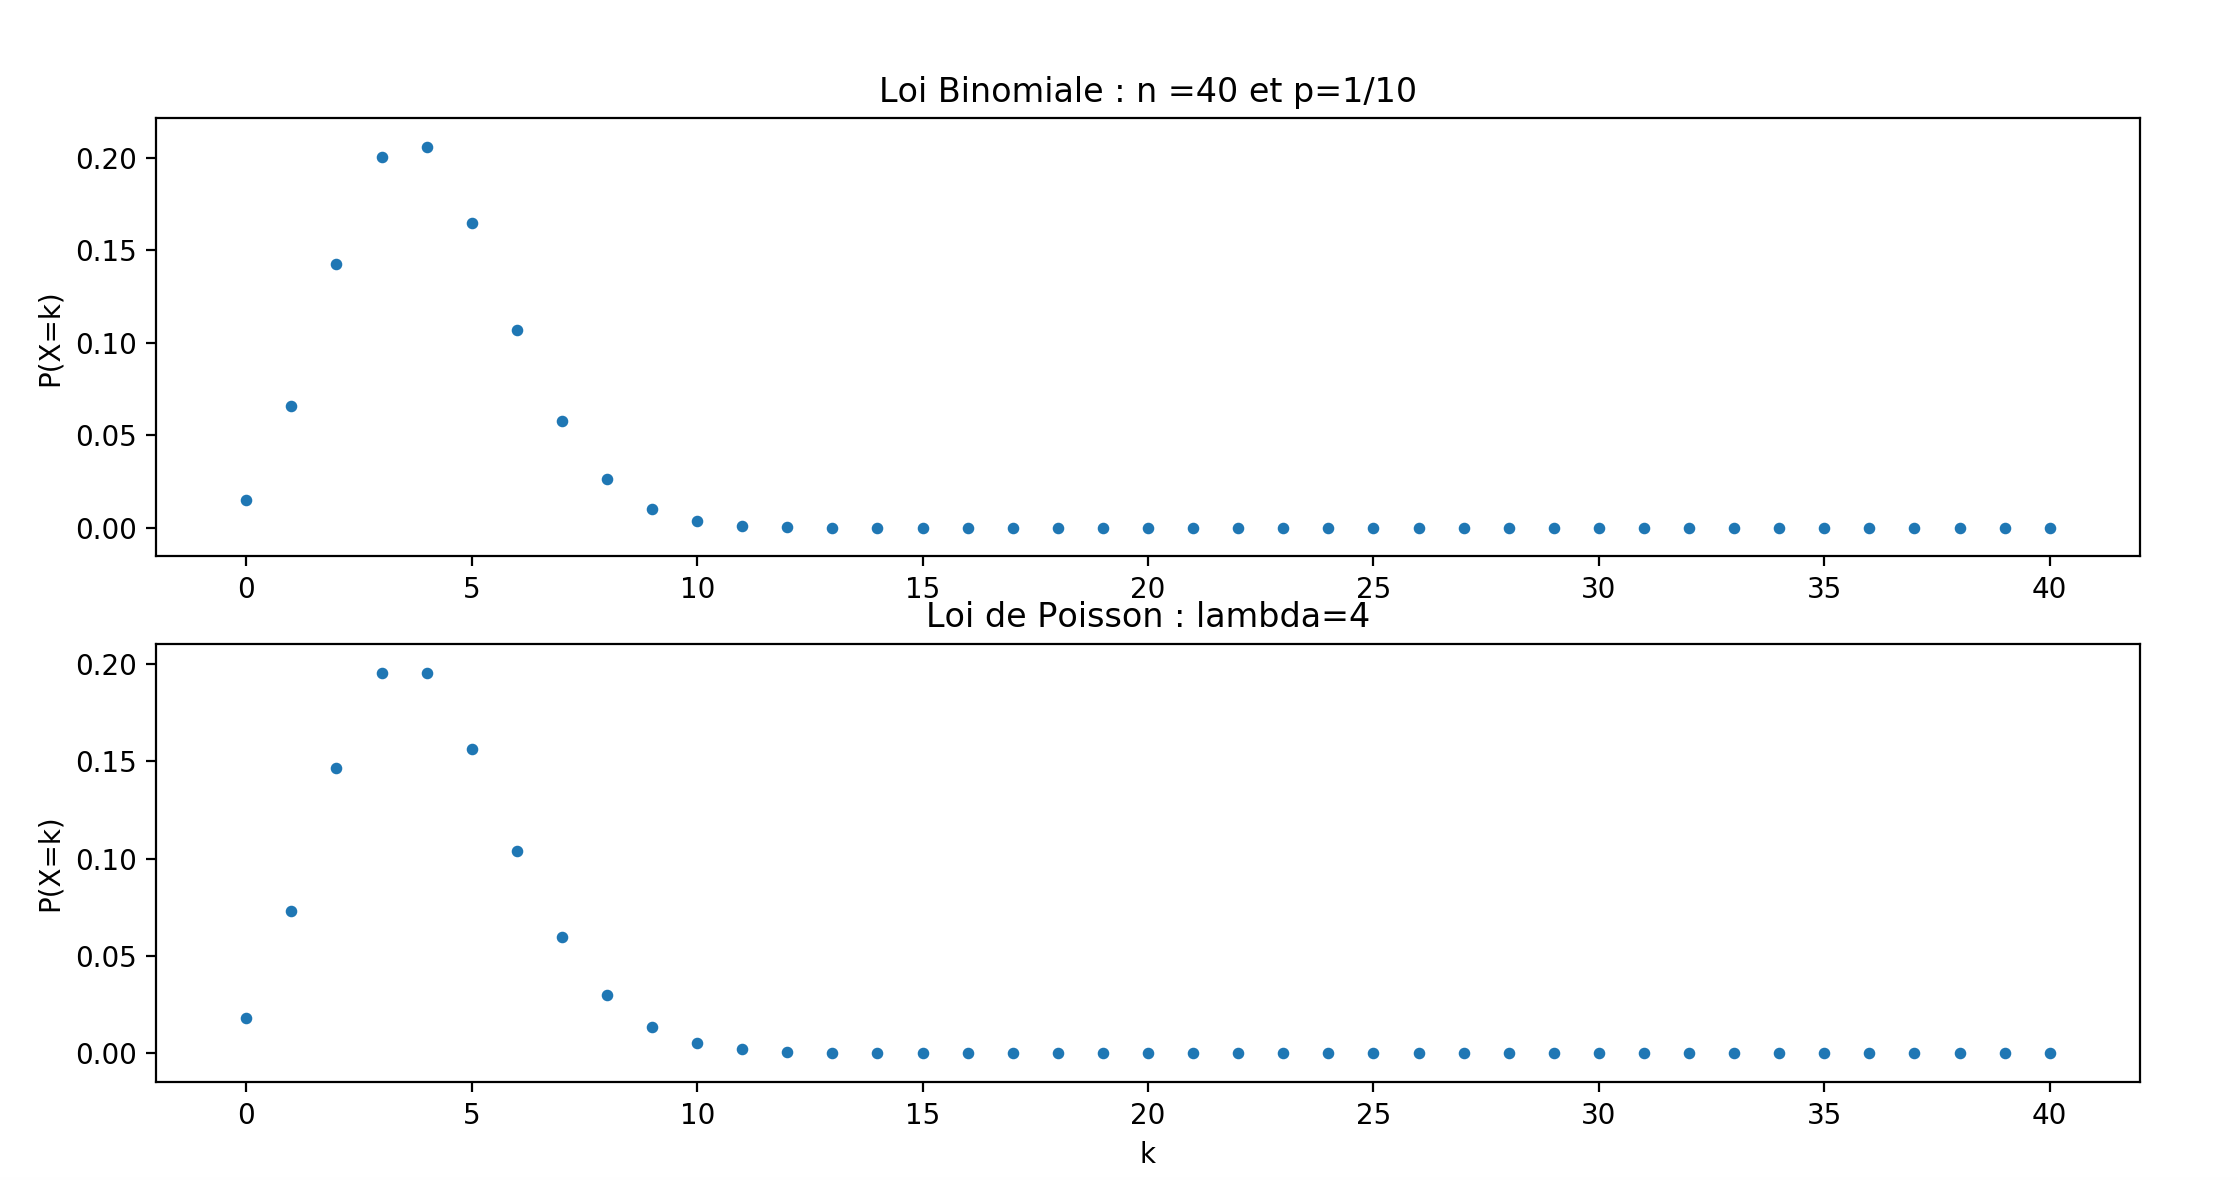
\includegraphics[scale=0.4]{Poisson}
\end{center}

\begin{ex}
On considère une assemblée de 500 personnes et on appelle $X$ la variable aléatoire égale au nombre de personnes nées un premier janvier. Quelle est la loi de $X$ ? Comment calculer la probabilité $\P(X=k)$ pour $k\in \Interv 0 5$ ?

\vspace{4cm}
\end{ex}

\section{Familles de variables aléatoires}
\subsection{Couple de variables aléatoires}

\begin{defip} Soient $X$ et $Y$ deux variables aléatoires sur $(\Omega, \mathcal{A})$. L'application :
$$ \omega \mapsto (X(\omega), Y(\omega))$$
est une variable aléatoire sur $(\Omega, \mathcal{A})$, appelée \textit{couple} $(X,Y)$.
\end{defip}

\begin{preuve}

\vspace{5cm}
\end{preuve}

\begin{notas}
\item Si $(x,y) \in X(\Omega) \times Y(\Omega)$, on note :
$$ ((X,Y)=(x,y))= (X=x,Y=y) = (X=x) \cap (Y=y)$$
\item Si $A \subset X(\Omega)$ et $B \subset Y(\Omega)$, on note :
$$ ((X,Y) \in (A \times B)) = (X \in A, Y \in B)= (X \in A) \cap (Y \in B)$$
\end{notas}

\begin{cor}[Admis] L'ensemble des variables aléatoires sur $(\Omega, \mathcal{A})$ à valeurs dans $\mathbb{K}$ est un $\mathbb{K}$-espace vectoriel (pour les lois usuelles).
\end{cor}

%\begin{preuve}
%
%\vspace{5cm}
%\end{preuve}

\begin{defin} Soit $(X,Y)$ une couple de variables aléatoires sur $(\Omega, \mathcal{A}, \P)$. 
\begin{itemize}
\item On appelle \textit{loi conjointe} de $X$ et $Y$ la loi du couple $(X,Y)$.
\item On appelle \textit{lois marginales} du couple $(X,Y)$ les lois de $X$ et $Y$.
\end{itemize}
\end{defin}

\begin{rem} On représente souvent la loi d'un couple dans un tableau (quand les supports sont finis) et on retrouve dans les marges les lois de $X$ et de $Y$ (donc les lois marginales).
\end{rem}

\begin{ex} On lance simultanément deux dés et on note $X$ le plus grand des deux chiffres obtenus et $Y$ le plus petit. Déterminer la loi conjointe de $X$ de $Y$. En déduire alors les lois marginales.

\vspace{10cm}
\end{ex}

\begin{prop} Soit $(X,Y)$ un couple de variables aléatoires sur $(\Omega, \mathcal{A}, \P)$.  La loi du couple détermine les lois marginales :

\begin{itemize}
\item $\dis \forall x \in X(\Omega), \, \P(X=x) = \sum_{y \in Y(\Omega)} P(X=x, Y=y) = \sum_{y \in Y(\Omega)} P(Y=y)P_{(Y=y)}(X=x)$.
\item $\dis \forall y \in Y(\Omega), \, \P(Y=x) = \sum_{x \in X(\Omega)} P(X=x, Y=y) = \sum_{x \in X(\Omega)} P(X=x)P_{(X=x)}(Y=y)$.
\end{itemize}
\end{prop}

\begin{preuve} Conséquence de la formule des probabilités totales.
%
%\vspace{3cm}
\end{preuve}
\medskip

\begin{att} La loi du couple $(X,Y)$ détermine ainsi les lois conjointes de $X$ et $Y$. La réciproque est fausse :

\vspace{5cm}
\end{att}

\begin{exa} On considère une urne qui contient deux boules blanches, une noire et une rouge. On tire simultanément deux boules dans cette urne et on note $X$ le nombre de boules blanches obtenues et $Y$ le nombre de boules noires tirées. Déterminer la loi du couple $(X,Y)$ puis les lois conjointes.
\end{exa}
\subsection{Conditionnement, indépendance}

\begin{defin}[Loi conditionnelle] Soient $X$ et $Y$ deux variables aléatoires sur $(\Omega, \mathcal{A}, \P)$ et $y \in Y(\Omega)$ tel que $\P(Y=y)>0$. La \textit{loi conditionnelle} de $X$ sachant $(Y=y)$ est l'application :
$$ \left\lbrace \begin{array}{ccl}
X(\Omega) & \longrightarrow & [0,1] \\
x & \longmapsto & P_{(Y=y)}(X=x) \\
\end{array}\right.$$
\end{defin}

\begin{ex} On considère six urnes numérotées de $1$ à $6$ et considère que l'urne $i \in \lbrace 1, \ldots, 6 \rbrace$ contient $i$ boules numérotées $1$ et $6-i$ boules numérotées $2$. On jette un dé équilibré et on pioche dans l'urne associé au chiffre obtenu avec le dé. On appelle $X$ le chiffre obtenu en lançant le dé et $Y$ le numéro de la boule obtenue. Quelle est la loi de $X$? Déterminer pour tout $i \in X(\Omega)$, la loi conditionnelle de $Y$ sachant que $(X=i)$. En déduire la loi de $Y$.

\vspace{10cm}
\end{ex}


\begin{defin}[Indépendance de deux variables aléatoires discrètes]
Soient $X$ et $Y$ deux variables aléatoires discrètes sur $(\Omega, \mathcal{A}, \P)$. On dit que $X$ et $Y$ sont \textit{indépendantes} si pour tout $(x,y) \in X(\Omega) \times Y(\Omega)$, les évènements $(X=x)$ et $(Y=y)$ sont indépendants, c'est-à-dire :
$$ P(X=x,Y=y)=P(X=x)P(Y=y)$$
\end{defin}

\begin{ex} Soient $X$ et $Y$ deux variables aléatoires à valeurs dans $\N$. On suppose que la loi conjointe de $X$ et $Y$ vérifie :
  \[
  \forall (j,k) \in \mathbb{N}^2,  \P( X = j,Y = k ) = \frac{a}{j!k!}
  \]
où $a \in \mathbb{R}$.
  \begin{enumerate}
  \item
    Déterminer la valeur de $a$.
    
    \vspace{4cm}
  \item
    Retrouvons les lois marginales de $X$ et $Y$.
    
    \vspace{5cm}
  \item
    Les variables $X$ et $Y$ sont elles indépendantes?
    
    \vspace{3cm}
  \end{enumerate}
\end{ex}

\begin{defin}[Indépendance de variables aléatoires discrètes]
Soit $I$ un ensemble d'indices et $(X_i)_{i \in I}$ une famille de variables aléatoires discrètes sur $(\Omega, \mathcal{A}, \P)$. On dit que les variables aléatoires $X_i$ (pour $i \in I$) sont \textit{mutuellement indépendantes} si pour toute famille $(x_i)_{i \in I}$ (avec $x_i \in X_i(\Omega)$), les évènements $(X_i=x_i)$ sont mutuellement indépendants, c'est-à-dire : pour toute famille finie $J \subset I$,
$$ P \left( \bigcap_{j \in J} (X_j=x_j) \right) = \prod_{j \in J} P(X_j=x_j)$$
\end{defin}


\begin{prop}[Admise] Soient $X$ et $Y$ deux variables aléatoires discrètes indépendantes sur $(\Omega, \mathcal{A}, \P)$.  Pour tous $A \subset X(\Omega)$ et $B \subset Y(\Omega)$, les évènements $(X \in A)$ et $(Y \in B)$ sont indépendants donc :
$$ \P(X \in A, Y \in B) = \P(X \in A) P(Y \in B)$$
\end{prop}



\begin{rem} On généralise cette propriété pour des variables aléatoires discrètes mutuellement indépendantes.
\end{rem}

\begin{ex} On considère deux joueurs $A$ et $B$ qui disposent chacun d'une pièce telle que la probabilité d'obtenir pile est $p \in ]0,1[$. Chaque joueur lance autant de fois que nécessaire sa pièce jusqu'à l'obtention d'un pile. On note $X_A$ (respectivement $X_B$) le nombre de lancers nécessaires au joueur $A$ (respectivement $B$) à l'obtention de son premier pile. On suppose que ces variables aléatoires sont indépendantes. 
\begin{enumerate}
\item Déterminons la loi de $X_A$ et $X_B$. 

\vspace{3cm}
\item Calculons la probabilité que les deux joueurs obtiennent leur premier pile après le même nombre de lancers.

\vspace{6cm}

\newpage

$\phantom{}$

\vspace{3cm}
\item On pose $Y=\max (X_A,X_B)$. Justifions que $Y(\Omega) = \mathbb{N}^*$ puis en notant $F_Y$ la fonction de répartition de $Y$, déterminons $F_Y(n)$ pour tout $n \in \mathbb{N}^*$. En déduire finalement la loi de $Y$.

\vspace{8cm}
\end{enumerate}
\end{ex}


\begin{cor} Soient $X$ et $Y$ deux variables aléatoires discrètes indépendantes sur $(\Omega, \mathcal{A}, \P)$.  Soient $f$ et $g$ deux fonctions définies respectivement sur $X(\Omega)$ et $Y(\Omega)$. Alors les variables aléatoires $f(X)$ et $g(Y)$ sont indépendantes.
\end{cor}

\begin{preuve}

\vspace{3cm}
\end{preuve}

\begin{ex} Si $X$ et $Y$ sont des variables aléatoires discrètes sur le même espace probabilité alors $\exp(X)$ et $Y+1$ sont indépendantes.
\end{ex}

\begin{prop} Soient $n \geq 2$, $p \in ]0,1[$ et $X_1, \ldots, X_n$ des variables aléatoires mutuellement indépendantes sur $(\Omega, \mathcal{A}, \P)$, suivant chacune la loi de Bernoulli de paramètre $p$. Alors la variable aléatoire $X_1+ \cdots + X_n$ suit la loi binomiale de paramètres $n$ et $p$.
\end{prop}

\begin{preuve}
\vspace{3cm}
\end{preuve}

\subsection{Un résultat d'existence}

\begin{thm} Soit $I$ un ensemble fini ou dénombrable. Considérons des lois $\mathcal{L}_i$ pour tout $i \in I$. Alors il existe un espace probabilisé $(\Omega, \mathcal{A}, \P)$ et une famille $(X_i)_{i \in I}$ de variables aléatoires sur cet espace probabilisé, mutuellement indépendantes, tels que pour tout $i \in I$, $X_i$ suit la loi $\mathcal{L}_i$.
\end{thm}

\begin{ex} Considérons un jeu de Pile ou Face, fini ou infini avec des lancers indépendants. Le résultat précédent qu'il existe des variables $X_n$ mutuellement indépendantes, définies sur le même espace probabilisé, tel que $X_n$ représente le lancer du $n$-ième lancer ($0$ pour Pile et $1$ pour Face par exemple).
\end{ex}







\section{Moments d'une variable aléatoire discrète}



\subsection{Espérance}


\begin{defin}[Espérance : cas fini]
Soit $X$ une variable aléatoire réelle sur $(\Omega, \mathcal{A}, \P)$ tel que $X(\Omega)$ est fini. On appelle \textit{espérance} de $X$ et on note $\E(X)$ le nombre :
 $$ \phantom{\E (X) = \sum_{x \in X(\Omega)}x  \P\big(X=x\big)}$$
\end{defin}

\begin{rems}
\item L'espérance est la \textit{moyenne} des valeurs possibles de $X$ pondérées par leurs probabilité.
\item Si $X(\Omega) = \{\liste x1n \}$, alors l'espérance de $X$ est donnée par la formule suivante :
 $$ \E(X) = x_1 P(X=x_1) + \cdots + x_n P(X=x_n)$$
\end{rems}

\begin{ex} Donnons l'espérance de la variable aléatoire $X$ dont la loi est donnée par :
$$\renewcommand{\arraystretch}{2.1}\begin{array}{|c||c|c|}
\hline
k & -4 & 6\\
\hline
\P(X=k) & \dis\tfrac 2 5 & \dis \tfrac 3 5\\
\hline
\end{array}$$

\vspace{2cm}
\end{ex}


\begin{defin}[Espérance : cas infini]
Soit $X$ une variable aléatoire discrète sur $(\Omega, \mathcal{A}, \P)$ donc le support est dénombrable. On peut écrire alors :
$$ X(\Omega) = \lbrace x_n \, \vert \, n \geq 0 \rbrace$$
On dit que $X$ \textit{admet une espérance} lorsque la série $\dis \sum_{n \geq 0} x_n P(X=x_n)$ est \textit{absolument convergente}.\\
Dans ce cas, cette série est convergente.\\
On appelle alors \textit{espérance} de $X$ et on note $\E(X)$ le réel défini par :
$$\E(X) = \sum\limits_{n = 0}^{+ \infty} x_n \P(X_n=x_n ) $$
\end{defin}

\noindent Si $X(\Omega)= \mathbb{N}$, alors on a (si l'espérance existe) :
$$\E(X) = \sum\limits_{k=0}^{+\infty} k \P(X=k)$$

\newpage

\begin{rem} On dit aussi que $X$ est d'espérance finie.
\end{rem}

\medskip

\begin{att} Contrairement à une variable aléatoire finie, une variable aléatoire discrète \textit{infinie} n'admet pas forcément d'espérance! Il faut prouver l'absolue convergence de la série avant de pouvoir parler d'espérance. 
\end{att}

\medskip

\begin{rems}
\item Dans le cas d'une variable aléatoire finie, l'espérance est une somme finie. Dans le cas d'une variable aléatoire discrète infinie, si \textit{l'espérance existe}, c'est la somme d'une série absolument convergente.
\item Une variable aléatoire finie admet \textit{toujours} une espérance.
\end{rems}

\begin{ex} Soit $X$ une variable aléatoire telle que $X(\Omega) = \mathbb{N}$ et telle que pour tout $n \in \mathbb{N}$, $\P(X=n)= \dfrac{1}{2^{n+1}} \cdot$

\noindent Justifier que cela définit bien une loi de probabilité. La variable $X$ admet-elle une espérance ? Si oui, calculer la.

\vspace{11.3cm}
\end{ex}

\begin{exa} Soit $X$ une variable aléatoire telle que $X(\Omega) = \mathbb{N}^*$ et telle que pour tout $n \in \mathbb{N}^*$, $\P(X=n)= \dfrac{1}{n}- \dfrac{1}{n+1} \cdot$

\noindent Justifier que cela définit bien une loi de probabilité. La variable $X$ admet-elle une espérance ? 
\end{exa}

\begin{prop}[Linéarité admise]
Soient $X$ et $Y$ deux variables aléatoires discrètes définies sur le même espace de probabilité, \textit{admettant une espérance} et $a$ un réel. Alors : 
\begin{itemize}
\item \textit{Linéarité :} $X+Y$ admet une espérance et $\E(X+Y) = \E(X)+\E(Y)$, $aX$ admet une espérance et $\E(aX)=a \E(X)$
\item \textit{Positivité :} Si $X$ est à valeurs positives, alors $\E(X) \geq 0 $
\item \textit{Croissance :} Si $X \le Y$, alors $\E(X) \leq \E(Y)$.
\end{itemize}
\end{prop}

\begin{preuve}

\vspace{5cm}
\end{preuve}

\begin{att} Pour utiliser la propriété de linéarité pour des variables discrètes infinies, il faut bien préciser que les variables admettent une espérance ce qui n'était pas nécessaire pour des variables aléatoires finies qui admettent toujours une espérance.
\end{att} 

\medskip


\begin{rems}
\item Si $X$ est une variable aléatoire discrète admettant une espérance et $a,b$ des réels. Alors 
$$ \E (aX + b) =a \E(X)+ b $$
\item Une variable aléatoire discrète est dite \textit{centrée} si elle admet une espérance et si son espérance est nulle
\end{rems}

%\begin{defip}
%\begin{itemize} 
%\item Une variable aléatoire discrète est dite \textit{centrée} si elle admet une espérance et si son espérance est nulle.
%\item Si une variable aléatoire discrète $X$ admet une espérance alors $X-\E(X)$ est une variable aléatoire discrète centrée.
%\end{itemize}
%\end{defip}

%\begin{prop}
%Soit $X$ une variable aléatoire discrète. Si $X$ admet une espérance, alors $X-\E(X)$ est une variable aléatoire discrète centrée.
%\end{prop}
%
%

\begin{prop} Soit $X$ une variable aléatoire sur $(\Omega, \mathcal{A}, \P)$ à valeurs dans $\mathbb{N}$. Alors la variable aléatoire $X$ admet une espérance si et seulement si la série :
$$ \dis \sum_{n \geq 1} \P(X \geq n)$$
converge et dans ce cas, l'espérance de $X$ est égale à la somme de cette série.
\end{prop}

\begin{preuve}
\vspace{10cm}
\end{preuve}

\begin{thm}[Espérances associées aux lois usuelles]
Soit $X$ une variable aléatoire sur $(\Omega, \mathcal{A}, \P)$. Soient $p \in ]0,1[$ et $\lambda \in \mathbb{R}_+^{*}$.

\begin{itemize}
\item Si $X$ suit une loi uniforme et que $X(\Omega)= \lbrace a_1, \ldots, a_n \rbrace$ alors $X$ admet une espérance et :
$$ \E(X) = \phantom{\dfrac{1}{n} \sum_{i = 1}^n a_i}$$
\item Si $X \hookrightarrow \mathcal{B}(p)$, $X$ admet une espérance et $\E(X)=$
\item Si $X \hookrightarrow \mathcal{B}(n,p)$, $X$ admet une espérance et $\E(X)=$
\item Si $X \hookrightarrow \mathcal{G}(p)$, $X$ admet une espérance et $\E(X)= $
\item Si $X \hookrightarrow \mathcal{P}(\lambda)$, $X$ admet une espérance et $\E(X)=$
\end{itemize}
\end{thm}

\newpage

$\phantom{}$
\begin{preuve}
\vspace{12cm}
\end{preuve}

\begin{rem} En particulier, si $X$ suit une loi uniforme sur $\Interv{1}{n}$, $\E(X) = \dfrac{n+1}{2} \cdot$
\end{rem}

\begin{prop}[Admise] Soient $X$ et $Y$ deux variables aléatoires discrètes indépendantes sur $(\Omega, \mathcal{A}, \P)$. Si ces deux variables admettent une espérance alors $XY$ aussi et $\E(XY)=\E(X)\E(Y)$.
\end{prop}
\subsection{Théorème de transfert}

\noindent Rappelons le Théorème de transfert (cas fini) : 


\begin{thm}[de transfert : cas fini]
Si $X$ une variable aléatoire finie sur $(\Omega, \mathcal{A}, \P)$ dont le support est de la forme $X(\Omega) = \{x_1, x_2, \ldots, x_n\}$ et $f$ une fonction dont le domaine de définition contient $X(\Omega)$ alors la variable aléatoire finie $f(X)$ admet une espérance et :
 $$ E(f(X)) = \sum_{x \in X(\Omega)} f(x) \P(X=x)$$
 \end{thm}

\begin{thm}[de transfert : cas infini]
Soient $X$ une variable aléatoire discrète infinie sur $(\Omega, \mathcal{A}, \P)$ et $f$ une fonction dont le domaine de définition contient $X(\Omega)$. On peut donc écrire :
$$ X(\Omega) = \lbrace x_n \, \vert \, n \geq 0 \rbrace$$
La variable aléatoire discrète $Y=f(X)$ admet une espérance \textit{si et seulement si} la série \linebreak $\dis \sum_{n \geq 0} f(x_n) P(X=x_n)$ est absolument convergente. \\
Dans ce cas, on a :
\[\E(Y)=\E\big(f(X)\big)= \sum_{n = 0}^{+ \infty} f(x_n) P(X=x_n)\]
\end{thm}

\begin{rem}
L'énorme intérêt du Théorème de transfert est de prouver l'existence et de calculer l'espérance de $Y=f(X)$ sans avoir besoin de déterminer la loi de $Y$, ce qui est parfois délicat.
\end{rem}

\begin{ex} Soit $X$ une variable aléatoire suivant une loi géométrique de paramètre $p \in ]0,1[$. Montrons que $X^2$ est d'espérance finie et déterminons cette espérance.

\vspace{10cm}
\end{ex}


\subsection{Variance et écart-type}
\begin{prop} Soit $X$ est une variable aléatoire discrète sur $(\Omega, \mathcal{A}, \P)$. Si $X^2$ admet une espérance alors $X$ admet une espérance.
\end{prop}

\begin{preuve}

\vspace{6cm}
\end{preuve}

\begin{defip}
Si $X$ est une variable aléatoire discrète sur $(\Omega, \mathcal{A}, \P)$  telle que $X^2$ a une espérance fini (on dit que $X$ a un \textit{moment d'ordre 2}), alors $X$ admet \textit{une variance}, notée $\V(X)$, qui est définie par :
$$\V(X) = \E\Big(\big(X-\E(X)\big)^2\Big)$$
Si $X$ admet une variance, alors on définit son \textit{écart-type} par 
$$\sigma (X) = \sqrt{\V(X)}$$
\end{defip}

\newpage

$\phantom{}$
\begin{preuve} 

\vspace{4cm}
\end{preuve}

\begin{rems} 
\item Si $X$ admet une variance, alors $X$ admet une espérance.
\item Une variable aléatoire finie admet toujours une variance.
\item $\V(X)$ mesure la dispersion de $X$ autour de son espérance.
\end{rems}

\begin{prop}[propriétés de la variance]
Soient $a$ et $b$ deux réels et $X$ est une variable aléatoire discrète admettant une variance. Alors :
\begin{itemize}
 \item $\V(X) \geq 0$ et $\sigma(X) \geq 0$;
 \item $aX+b$ admet une variance, et :  
$$\V(aX+b) = \phantom{a^2 \V(X)} \et \sigma(aX+b) = \phantom{\vert a \vert \sigma(X)} $$
\end{itemize}
\end{prop}

\begin{preuve}

\vspace{5cm}
\end{preuve}

\begin{prop}[Formule de Koenig-Huygens]
Si $X$ admet une variance, alors :
$$\V(X) = \phantom{\E\big(X^2\big) - \big(\E(X)\big)^2}$$
\end{prop}

\begin{preuve}
\vspace{3cm}
\end{preuve}

\begin{metho} 
La formule de Koenig-Huygens est souvent utilisée pour calculer $\V(X)$ : on calcule $\E(X^2)$ à l'aide du {théorème de transfert} : \textit{en cas de convergence absolue}, on a : 
$$\E(X^2)=\sum\limits_{x\in X(\Omega)} x^2  \P(X=x)$$
\end{metho}

\begin{thm}[Variances associées aux lois usuelles]
Soit $X$ une variable aléatoire discrète sur $(\Omega, \mathcal{A}, \P)$. Soit $p \in ]0,1[$ et $\lambda \in \mathbb{R}_+^{*}$.

\begin{itemize}
\item Si $X \hookrightarrow \mathcal{B}(p)$, $X$ admet une variance et $\V(X)=$
\item Si $X \hookrightarrow \mathcal{B}(n,p)$, $X$ admet une variance et $\V(X)=$
\item Si $X \hookrightarrow \mathcal{G}(p)$, $X$ admet une variance et $\V(X)= $
\item Si $X \hookrightarrow \mathcal{P}(\lambda)$, $X$ admet une variance et $\V(X)= $
\end{itemize}
\end{thm}

\begin{preuve}

\vspace{15cm}
\end{preuve}

\begin{rem} Si $X$ suit la loi uniforme sur $\Interv{1}{n}$ alors $X$ admet une variance et $\V(X) = \dfrac{n^2-1}{12} \cdot$
\end{rem} 

\begin{ex} Déterminons la variance de la variable $X$ dont la loi est donnée par :
$$\renewcommand{\arraystretch}{2.1}\begin{array}{|c||c|c|}
\hline
k & -4 & 6\\
\hline
\P(X=k) & \dis\frac 2 5 & \dis \frac 3 5\\
\hline
\end{array}$$

\vspace{4cm}
\end{ex}

\subsection{Covariance et corrélation}

\begin{prop}[Inégalité de Cauchy-Schwarz]
Soient $X$ et $Y$ deux variables aléatoires discrètes sur $(\Omega, \mathcal{A}, \P)$ admettant une variance. Alors $XY$ admet une espérance et :
$$ \vert \E(XY) \vert \leq \sqrt{\E(X^2)\E(Y^2)}$$
\end{prop}

\begin{preuve}
\vspace{3cm}
\end{preuve}


\begin{defip} 
Soient $X$ et $Y$ deux variables aléatoires discrètes sur $(\Omega, \mathcal{A}, \P)$ admettant une variance.
\begin{itemize}
\item La variable $(X-\E(X))(Y-\E(Y))$ admet une espérance que l'on appelle la \textit{covariance} de $X$ et $Y$ et que l'on note $\textrm{Cov}(X,Y)$. On a de plus :
$$ \textrm{Cov}(X,Y) = \E((X-\E(X))(Y-\E(Y))) = \E(XY) - \E(X)\E(Y)$$
\item Si $\sigma(X)$ et $\sigma(Y)$ sont non nuls, on appelle \textit{coefficient de corrélation} de $X$ et $Y$, et on note $\rho(X,Y)$, le réel :
$$ \rho(X,Y) = \dfrac{\textrm{Cov}(X,Y)}{\sigma(X) \sigma(Y)}$$
\end{itemize}
\end{defip}

\begin{preuve}
\vspace{6cm}
\end{preuve}

\begin{rems}
\item Si $X$ admet une variance, $\textrm{Cov}(X,X)= \textrm{V}(X)$.
\item La covariance est symétrique : si $X$ et $Y$ admettent des variances, $\textrm{Cov}(X,Y) = \textrm{Cov}(Y,X)$. On peut montrer que la covariance est linéaire par rapport à la première variable.
\end{rems}

\begin{prop} Soient $X$ et $Y$ deux variables aléatoires indépendantes sur $(\Omega, \mathcal{A}, \P)$ admettant une variance. Alors $\textrm{Cov}(X,Y)=0$. La réciproque est fausse.
\end{prop}

\begin{preuve}

\vspace{1cm}
\end{preuve}

\begin{exa} Soient $X$ une variable suivant une loi uniforme sur $\lbrace -1,0,1 \rbrace$ et $Y=X^2$. Justifier que $\textrm{Cov}(X,Y)=0$ (on pourra remarquer que $XY=X$). Montrer que $X$ et $Y$ ne sont pas indépendantes (calculer par exemple $\P(X=0, Y=1)$).
\end{exa}

\begin{prop} Soient $X$ et $Y$ deux variables aléatoires sur $(\Omega, \mathcal{A}, \P)$ admettant une variance. Alors :
$$ \vert \textrm{Cov}(X,Y) \vert \leq \sigma(X) \sigma(Y)$$
et en particulier si $\sigma(X)$ et $\sigma(Y)$ sont non nuls, 
$$ \rho(X,Y) \in [-1,1]$$
\end{prop}

\begin{preuve}

\vspace{4cm}
\end{preuve}

\begin{rem} Le coefficient de corrélation $\rho(X,Y)$ \og mesure la dépendance \fg entre $X$ et $Y$. Si $X$ et $Y$ sont indépendantes, ce coefficient est nul et si il est proche de $1$ en valeur absolue, il y a une \og dépendance affine \fg entre $X$ et $Y$ (conséquence de l'inégalité de Cauchy-Schwarz).
\end{rem}

\begin{prop}[Variance d'une somme de variables aléatoires discrètes]
Soient $n \geq 2$ et $X_1, \ldots, X_n$ des variables aléatoires sur $(\Omega, \mathcal{A}, \P)$, admettant une variance. Alors :
\begin{itemize}
\item $X_1 + \cdots + X_n = \dis \sum_{k=1}^n X_k$ admet une variance et :
$$ \textrm{V} \left(\sum_{k=1}^n X_k \right) = \sum_{k=1}^n \textrm{V}(X_k) + 2 \sum_{1\leq i<j \leq n} \textrm{Cov}(X_i,X_j)$$
\item Si de plus les variables sont deux à deux indépendantes, on a :
$$ \textrm{V} \left(\sum_{k=1}^n X_k \right) = \sum_{k=1}^n \textrm{V}(X_k)$$
\end{itemize}
\end{prop}

\begin{preuve}
\vspace{10cm}
\end{preuve}

\begin{rem} On retrouve l'expression de la variance d'une variable aléatoire suivant une loi binomiale.

\vspace{5cm}
\end{rem}

\section{Variables aléatoires à valeurs dans $\mathbb{N}$}
\subsection{Fonctions génératrices}
\begin{defip} Soit $X$ une variable aléatoire sur $(\Omega, \mathcal{A}, \P)$ à valeurs dans $\mathbb{N}$.

\noindent Pour tout $t \in [-1,1]$, la variable aléatoire $t^X$ admet une espérance. On pose alors pour tout $t \in [-1,1]$,
$$ G_X(t)= \E(t^X) = \sum_{n=0}^{+ \infty} \P(X=n) t^n$$
La fonction $G_X$ est la somme d'une série entière de rayon de convergence supérieur ou égal à $1$. On l'appelle la \textit{fonction génératrice} de $X$.
\end{defip}

\begin{preuve}
\vspace{5cm}
\end{preuve}

\begin{rems}
\item $G_X(1)= \dis \sum_{n=0}^{+ \infty} \P(X=n)=1$.
\item Si $X(\Omega)$ est fini, $G_X$ est un polynôme.
\end{rems}

\begin{ex} Déterminons les fonctions génératrices de variables suivant une loi de Bernoulli et une loi binomiale.

\vspace{5cm}
\end{ex}

\begin{prop} La loi d'une variable est déterminée par sa fonction génératrice : si $X$ et $Y$ sont deux variables aléatoires sur $(\Omega, \mathcal{A}, \P)$, ayant le même support et telles que :
$$ \exists r \in ]0,1], \; \forall t \in ]-r,r[, \; G_X(t)=G_Y(t)$$
Alors $X$ et $Y$ ont la même loi.
\end{prop}

\begin{preuve}

\vspace{3cm}
\end{preuve}

\begin{rem} D'après l'expression des coefficients d'une série entière, on a :
$$ \forall n \in \mathbb{N}, \; P(X=n) = \dfrac{G_X^{(n)}(0)}{n!}$$
\end{rem}

\begin{prop}[Fonctions génératrices associées aux lois usuelles]
Soit $X$ une variable aléatoire sur $(\Omega, \mathcal{A}, \P)$. Soit $p \in ]0,1[$ et $\lambda \in \mathbb{R}_+^{*}$.

\begin{itemize}
\item Si $X \hookrightarrow \mathcal{B}(p)$, alors pour tout $t \in \mathbb{R}$, $G_X(t)=1-p+pt$.
\item Si $X \hookrightarrow \mathcal{B}(n,p)$,  alors pour tout $t \in \mathbb{R}$, $G_X(t)=(1-p+pt)^n$.
\item Si $X \hookrightarrow \mathcal{G}(p)$,  alors pour tout $t \in \mathbb{R}$, $G_X(t)=\dfrac{pt}{1-(1-p)t}\cdot$
\item Si $X \hookrightarrow \mathcal{P}(\lambda)$,  alors pour tout $t \in \mathbb{R}$, $G_X(t)=e^{\lambda(t-1)}$.
\end{itemize}
\end{prop}

\begin{preuve}

\vspace{10cm}
\end{preuve}

\subsection{Lien avec l'espérance et la variance}

\begin{prop}[Lien entre fonction génératrice et espérance] Soit $X$ une variable aléatoire sur $(\Omega, \mathcal{A}, \P)$ à valeurs dans $\mathbb{N}$. Les assertions suivantes sont équivalentes :

\begin{itemize}
\item $X$ admet une espérance.
\item $G_X$ est dérivable à gauche en $1$.
\end{itemize}
Si les assertions sont vérifiées, on a $G_X'(1)=\E(X)$.
\end{prop}

\begin{rem} On peut retrouver facilement cette égalité :

\vspace{3cm}
\end{rem}

\begin{ex} Retrouvons les valeurs des espérances de variables suivant des lois de bernoulli et binomiale :

\vspace{5cm}
\end{ex}

\begin{exa} Retrouver les valeurs des espérances de variables suivant des lois géométriques et de Poisson.
\end{exa}
\begin{prop}[Lien entre fonction génératrice et variance] Soit $X$ une variable aléatoire sur $(\Omega, \mathcal{A}, \P)$ à valeurs dans $\mathbb{N}$. Les assertions suivantes sont équivalentes :

\begin{itemize}
\item $X$ admet une variance.
\item $G_X$ est deux fois dérivable à gauche en $1$.
\end{itemize}
Si les assertions sont vérifiées, on a $\V(X)=G_X''(1)+G_X'(1)-G_X'(1)^2$.
\end{prop}

\begin{rem} On peut retrouver facilement cette égalité :

\vspace{4cm}
\end{rem}

\begin{ex} Retrouvons les valeurs des variances de variables suivant des lois de Bernoulli et binomiale :

\vspace{5cm}
\end{ex}

\begin{exa} Retrouver les valeurs des variances de variables suivant des lois géométriques et de Poisson.
\end{exa}

\subsection{Fonctions génératrices et somme}

\begin{prop}[Fonction génératrice d'une somme de variables aléatoires discrètes]
Soient $X$ et $Y$ deux variables aléatoires indépendantes sur $(\Omega, \mathcal{A}, \P)$ à valeurs dans $\mathbb{N}$. Alors pour tout $t \in [-1,1]$,
$$ G_{X+Y}(t) = G_X(t) G_Y(t)$$
\end{prop}

\begin{preuve}

\vspace{3cm}
\end{preuve}

\begin{cor} Soient $X$ et $Y$ deux variables aléatoires indépendantes sur $(\Omega, \mathcal{A}, \P)$ et $(\lambda, \mu) \in (\mathbb{R}_+^{*})^2$. On suppose que $X \hookrightarrow \mathcal{P}(\lambda)$ et $Y \hookrightarrow \mathcal{P}(\mu)$. Alors $X+Y \hookrightarrow \mathcal{P}(\lambda+\mu)$
\end{cor}

\begin{preuve}

\vspace{5cm}
\end{preuve}

\begin{exa} Soient $n \geq 1$ et $(p,q) \in ]0,1[^2$. Montrer que si $X \hookrightarrow \mathcal{B}(n,p)$ et $Y \hookrightarrow \mathcal{B}(n,q)$ et que $X$ et $Y$ sont indépendantes alors $X+Y \hookrightarrow \mathcal{B}(n,p+q)$.
\end{exa}

\section{Estimations, résultats asymptotiques}

\begin{thm}[Inégalité de Markov]
Soit $X$ une variable aléatoire discrète positive sur $(\Omega, \mathcal{A}, \P)$ et admettant une espérance. Alors pour tout $\varepsilon>0$,
$$ \P(X \geq \varepsilon) \leq \dfrac{\E(X)}{\varepsilon}$$
\end{thm}

\begin{preuve}

\vspace{5cm}
\end{preuve}

\begin{thm}[Inégalité de Bienaymé-Tchebychev]
Soit $X$ une variable aléatoire discrète sur $(\Omega, \mathcal{A}, \P)$ et admettant une variance. Alors pour tout $\varepsilon>0$,
$$ \P( \vert X- \E(X) \vert \geq \varepsilon) \leq \dfrac{\V(X)}{\varepsilon^2}$$
\end{thm}

\begin{preuve}
\vspace{5cm}
\end{preuve}

\begin{rem} Plus la variance est petite, plus la probabilité que la variable s'écarte de son espérance est petite.
\end{rem}

\begin{ex} Soit $X$ une variable aléatoires réelle discrète admettant une variance $\sigma^{2}$ (avec $\sigma > 0$). Montrons que :
  \[
  \forall \alpha > 0,\:\P\left(\vert X - \E(X) \vert < \alpha \sigma \right) \geq 1 - \frac{1}{\alpha^{2}}
  \]
  
 \vspace{5cm}
\end{ex}

\begin{thm}[Loi faible des grands nombres] Soit $(X_n)_{n \geq 1}$ une suite de variable aléatoires discrètes sur $(\Omega, \mathcal{A}, \P)$. On suppose que :
\begin{itemize}
\item Les variables aléatoires $X_n$ sont deux à deux indépendantes.
\item Les variables aléatoires $X_n$ ont la même loi et admettent une variance.
\end{itemize}
On note alors $m$ et $\sigma$, les espérances et écart-types communs, et on pose pour tout $n \geq 1$,
$$ S_n = X_1 + \cdots + X_n$$
Alors pour tout $\varepsilon>0$,
$$ \P \left( \left\vert \dfrac{S_n}{n}-m \right\vert  \geq \varepsilon \right) \leq \dfrac{\sigma^2}{n \varepsilon^2}$$
et en particulier :
$$ \lim_{n \rightarrow + \infty} \P \left( \left\vert \dfrac{S_n}{n}-m \right\vert  \geq \varepsilon \right) = 0$$
\end{thm}

\begin{preuve}

\vspace{8cm}
\end{preuve}

\newpage

\phantom{test}

\vspace{6cm}
\begin{rems} 
\item Supposons que l'on répète une infinité de fois la même expérience où l'on observe un résultat. On peut modéliser cette situation par des variables aléatoires $X_n$ où pour tout $n \geq 1$, $X_n$ représente le résultat observé à la $n$-ième répétition de cette expérience. On peut modéliser ceci en supposant que les variables $X_n$ sont deux à deux indépendantes. Dans ce cas, $\dfrac{S_n}{n}$ représente la moyenne des résultats lors des $n$ premières répétitions de l'expérience. Ainsi, le résultat précédent affirme que pour tout nombre $\varepsilon>0$, la probabilité que $\dfrac{S_n}{n}$ s'écarte de l'espérance commune $m$ d'au moins $\varepsilon$ tend vers $0$ plus le nombre d'expériences est grand. Par passage à l'évènement contraire, on a :
$$ \P \left( m - \varepsilon < \dfrac{S_n}{n}< m + \varepsilon \right) \underset{n \rightarrow + \infty}{\longrightarrow} 1$$
\item Ce théorème permet parfois de vérifier un modèle : si par exemple, on suppose une pièce équilibrée et que les répétitions du lancer de cette pièce nous donne une moyenne ne tendant pas vers $\dfrac{1}{2}$, il faut surement repenser le modèle.
\end{rems}

\medskip

\noindent Voici un exemple pour finir : on représente ici trois simulations de 800 lancers d'une pièce équilibrée et on représente la fréquence relative d'apparition du Face :

\begin{center}
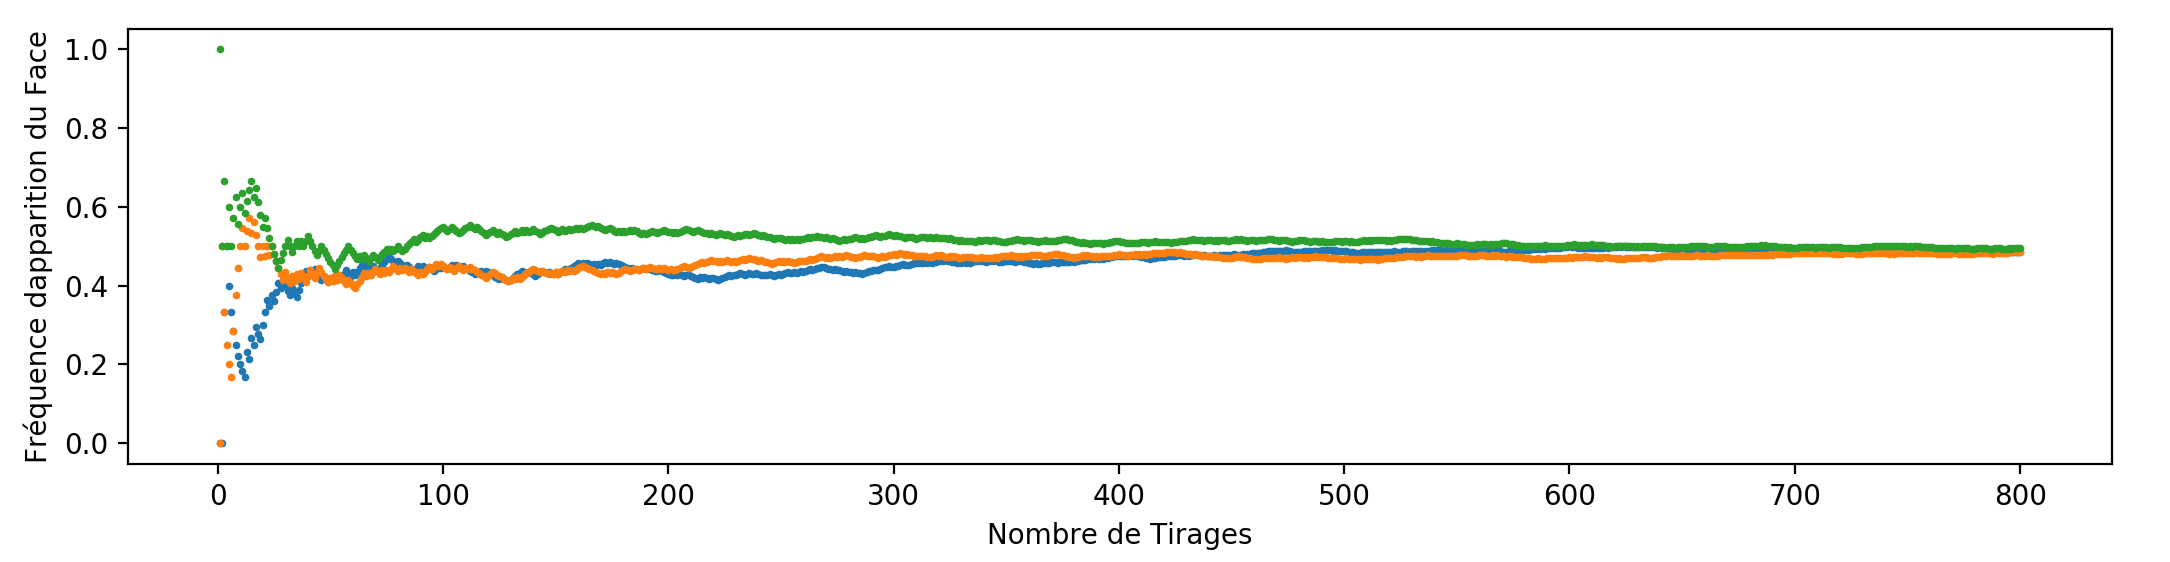
\includegraphics[scale=0.5]{Face}
\end{center}


\end{document}
